%%%%%%%%%%%%%%%%%%%%%%% file template.tex %%%%%%%%%%%%%%%%%%%%%%%%%
%
% This is a general template file for the LaTeX package SVJour3
% for Springer journals.          Springer Heidelberg 2010/09/16
%
% Copy it to a new file with a new name and use it as the basis
% for your article. Delete % signs as needed.
%
% This template includes a few options for different layouts and
% content for various journals. Please consult a previous issue of
% your journal as needed.
%
%%%%%%%%%%%%%%%%%%%%%%%%%%%%%%%%%%%%%%%%%%%%%%%%%%%%%%%%%%%%%%%%%%%
%
% First comes an example EPS file -- just ignore it and
% proceed on the \documentclass line
% your LaTeX will extract the file if required
\begin{filecontents*}{example.eps}
%!PS-Adobe-3.0 EPSF-3.0
%%BoundingBox: 19 19 221 221
%%CreationDate: Mon Sep 29 1997
%%Creator: programmed by hand (JK)
%%EndComments
gsave
newpath
  20 20 moveto
  20 220 lineto
  220 220 lineto
  220 20 lineto
closepath
2 setlinewidth
gsave
  .4 setgray fill
grestore
stroke
grestore
\end{filecontents*}
%
\RequirePackage{fix-cm}
%
%\documentclass{svjour3}                     % onecolumn (standard format)
%\documentclass[smallcondensed]{svjour3}     % onecolumn (ditto)
\documentclass[smallextended]{svjour3}       % onecolumn (second format)
%\documentclass[twocolumn]{svjour3}          % twocolumn
%
\smartqed  % flush right qed marks, e.g. at end of proof
%
\usepackage{graphicx}
\usepackage{amssymb}
\usepackage{amsmath}
%
% \usepackage{mathptmx}      % use Times fonts if available on your TeX system
%
% insert here the call for the packages your document requires
%\usepackage{latexsym}
% etc.
%
% please place your own definitions here and don't use \def but
% \newcommand{}{}
%
% Insert the name of "your journal" with
% \journalname{myjournal}
%
\begin{document}

\title{Narrowing the condition for the existance of Collatz Cycles%\thanks{Grants or other notes
%about the article that should go on the front page should be
%placed here. General acknowledgments should be placed at the end of the article.}
}
\subtitle{Do you have a subtitle?\\ If so, write it here}

%\titlerunning{Short form of title}        % if too long for running head

\author{Christian Koch         \and
        Eldar Sultanow
}

%\authorrunning{Short form of author list} % if too long for running head

\institute{C. Koch \at
              first address \\
              Tel.: +123-45-678910\\
              Fax: +123-45-678910\\
              \email{fauthor@example.com}           %  \\
%             \emph{Present address:} of F. Author  %  if needed
           \and
           E. Sultanow \at
              second address
}

\date{Received: date / Accepted: date}
% The correct dates will be entered by the editor


\maketitle

\begin{abstract}
Insert your abstract here. Include keywords, PACS and mathematical
subject classification numbers as needed.
\keywords{First keyword \and Second keyword \and More}
% \PACS{PACS code1 \and PACS code2 \and more}
% \subclass{MSC code1 \and MSC code2 \and more}
\end{abstract}

\section{Introduction}
\label{intro}
The Collatz conjecture is one of the unsolved "Million Buck Problems" \cite{Ref_Williams_2000}. When Lothar Collatz began his professorship in Hamburg in 1952, he mentioned this problem to his colleague Helmut Hasse. From 1976 to 1980, Collatz wrote several letters but missed referencing that he first proposed the problem in 1937. He introduced a function $g:\mathbb{N}\rightarrow\mathbb{N}$ as follows:
\begin{equation}
\label{eq:func_collatz}
g(x)=
\begin{cases}
3x+1	&	2\nmid x\\
x/2		&	\text{otherwise}
\end{cases}
\end{equation}

This function is surjective, but it is not injective (for example $g(3)=g(20))$ and thus is not reversible. The Collatz conjecture states that for each start number $x_1>0$ the sequence $x_1,x_2=g(x_1),x_3=g(x_2),\ldots$ will at some point enter the so called trivial cycle $1,4,2$. One example is the sequence $17,52,26,13,40,20,10,5,16,8,4,2,1$ starting at $x_1=17$. The assumption has not yet been proven. If the conjecture were wrong, then for a starting number $x_1$ the sequence either would diverge indefinitely or enter a cycle different from the trivial one (a so called non-trivial cycle). Subject of our investigation are the non-trivial cycles and the question if these cycles are possible, under which condition they might occur and which cycles can be considered to be impossible.
For this we define a more convenient function opting out all even integers from Collatz sequences:
\begin{equation}
\label{eq:func_collatz_odd}
f(x)=(3x+1)\cdot2^{-\alpha(x)}
\end{equation}
Note that $\alpha(x)$ is the largest possible exponent for which $2^{\alpha(x)}$ divides $3x+1$.

\section{Related Research}
\label{sec:1}
Hercher \cite{Ref_Hercher_2018} dealed with conditions for a cycle and showed that a .

\section{Defining the conditions for cycles}
\label{sec:1}
Text with citations \cite{RefB} and \cite{RefJ}.
\subsection{Subsection title}
\label{sec:2}
as required. Don't forget to give each section
and subsection a unique label (see Sect.~\ref{sec:1}).
\paragraph{Paragraph headings} Use paragraph headings as needed.
\begin{equation}
a^2+b^2=c^2
\end{equation}

% For one-column wide figures use
\begin{figure}
% Use the relevant command to insert your figure file.
% For example, with the graphicx package use
  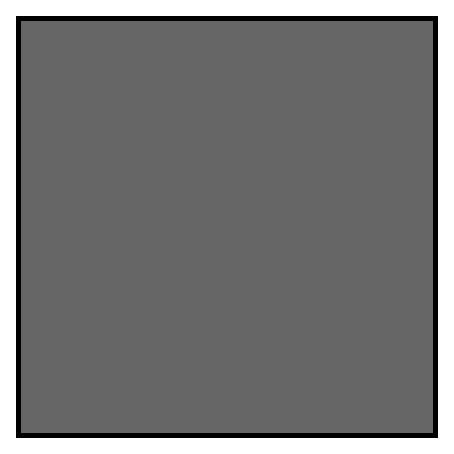
\includegraphics{example.eps}
% figure caption is below the figure
\caption{Please write your figure caption here}
\label{fig:1}       % Give a unique label
\end{figure}
%
% For two-column wide figures use
\begin{figure*}
% Use the relevant command to insert your figure file.
% For example, with the graphicx package use
  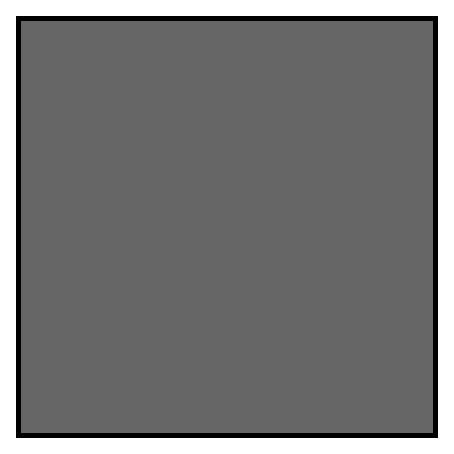
\includegraphics[width=0.75\textwidth]{example.eps}
% figure caption is below the figure
\caption{Please write your figure caption here}
\label{fig:2}       % Give a unique label
\end{figure*}
%
% For tables use
\begin{table}
% table caption is above the table
\caption{Please write your table caption here}
\label{tab:1}       % Give a unique label
% For LaTeX tables use
\begin{tabular}{lll}
\hline\noalign{\smallskip}
first & second & third  \\
\noalign{\smallskip}\hline\noalign{\smallskip}
number & number & number \\
number & number & number \\
\noalign{\smallskip}\hline
\end{tabular}
\end{table}


%\begin{acknowledgements}
%If you'd like to thank anyone, place your comments here
%and remove the percent signs.
%\end{acknowledgements}


% Authors must disclose all relationships or interests that 
% could have direct or potential influence or impart bias on 
% the work: 
%
% \section*{Conflict of interest}
%
% The authors declare that they have no conflict of interest.


% BibTeX users please use one of
%\bibliographystyle{spbasic}      % basic style, author-year citations
%\bibliographystyle{spmpsci}      % mathematics and physical sciences
%\bibliographystyle{spphys}       % APS-like style for physics
%\bibliography{}   % name your BibTeX data base

% Non-BibTeX users please use
\begin{thebibliography}{}
%
% and use \bibitem to create references. Consult the Instructions
% for authors for reference list style.
%
% Format for Journal Reference
% Author, Article title, Journal, Volume, page numbers (year)
% Format for books
% Author, Book title, page numbers. Publisher, place (year)
\bibitem{Ref_Williams_2000}
S. W. Williams, Million Buck Problems, National Association of Mathematicians Newsletter, 31(2), 1-3 (2000)

\bibitem{Ref_Hercher_2018}
C. Hercher, Über die Länge nicht-trivialer Collatz-Zyklen, Die Wurzel, 6-7, 1-13 (2018)

% Format for books
\bibitem{RefB}
Author, Book title, page numbers. Publisher, place (year)
% etc
\end{thebibliography}

\end{document}
% end of file template.tex

